Before we start with the characterization of the fiber weveral verification tasks must be performed to verify that the system is working properly. The quality of the tightness to the light of the black box used and the correct operation of the PMT for this study, which involves checking the correct operation of the PCB designed and checking the linearity of the PMT output signal in the study range, must be verified.

First, the quality of the light tightness of the black box used was verified. It is important because we are detecting small signals, a few hundred photons per nanosecond, so it must be verified that the background of the system are below that.

This test is performed by measuring a no-clad fiber, whose length is $20~\cm$, in the previous assembly. This measurement was carried out by feeding the LED with four different intensities ($0.05~\milli\ampere$, $0.1~\milli\ampere$, $0.15~\milli\ampere$ and $0.2~\milli\ampere$) and this measurement will be repeated covering the set up with a special black blanket from Thorlabs \cite{BlackBlancket}, with which it can be ensured that the amount of external photons that reach that system is negligible. 

This test was repeated for three different no clad fiber samples and the mean and standard deviation were calculated using the equations \ref{eq:MeanAndStandardDesviation} for each light intensity.

\begin{equation}
\bar{x}=\frac{\sum_{i=0}^{N}x_i}{N}; \qquad Std.~Des. = \frac{\sqrt{\sum_{i=0}^{N}(x_i-\bar{x})^2}}{N-1};
\label{eq:MeanAndStandardDesviation}
\end{equation}

The difference between the results obtained in both tests is presented in Figure \ref{fig:LightTightnessTest}.

%\begin{figure}[]
 %\centering
  %\subfloat[The measurement obtained by covering the setup with a special black blanket and not covering.]{
   %\label{subfig:LightTightnessTestData}
    %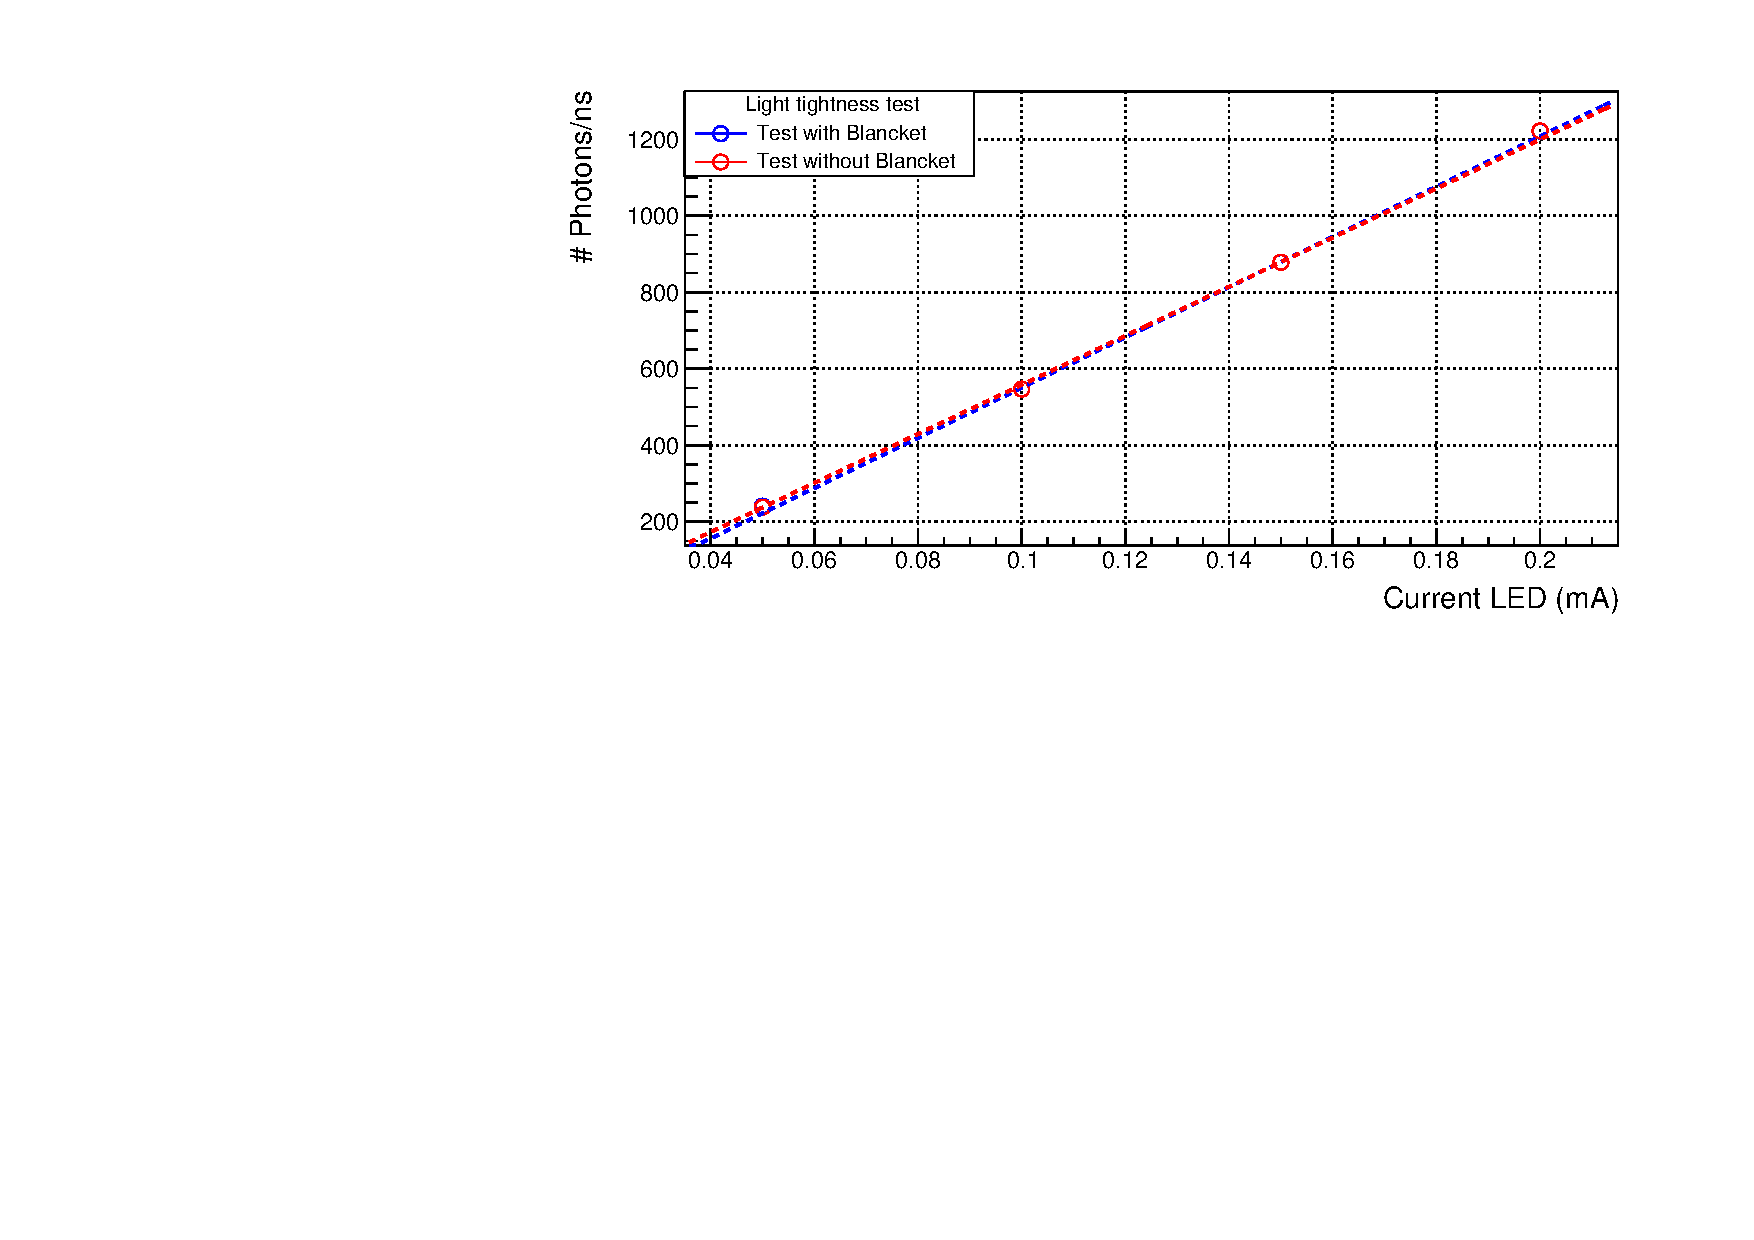
\includegraphics[width=0.9\textwidth]{4ResearchAndDevelopments/41Fibers/Light_tightness_Measurements.pdf}}
    %\newline
  %\subfloat[.]{
   %\label{subfig:LightTightnessTestDifference}
    %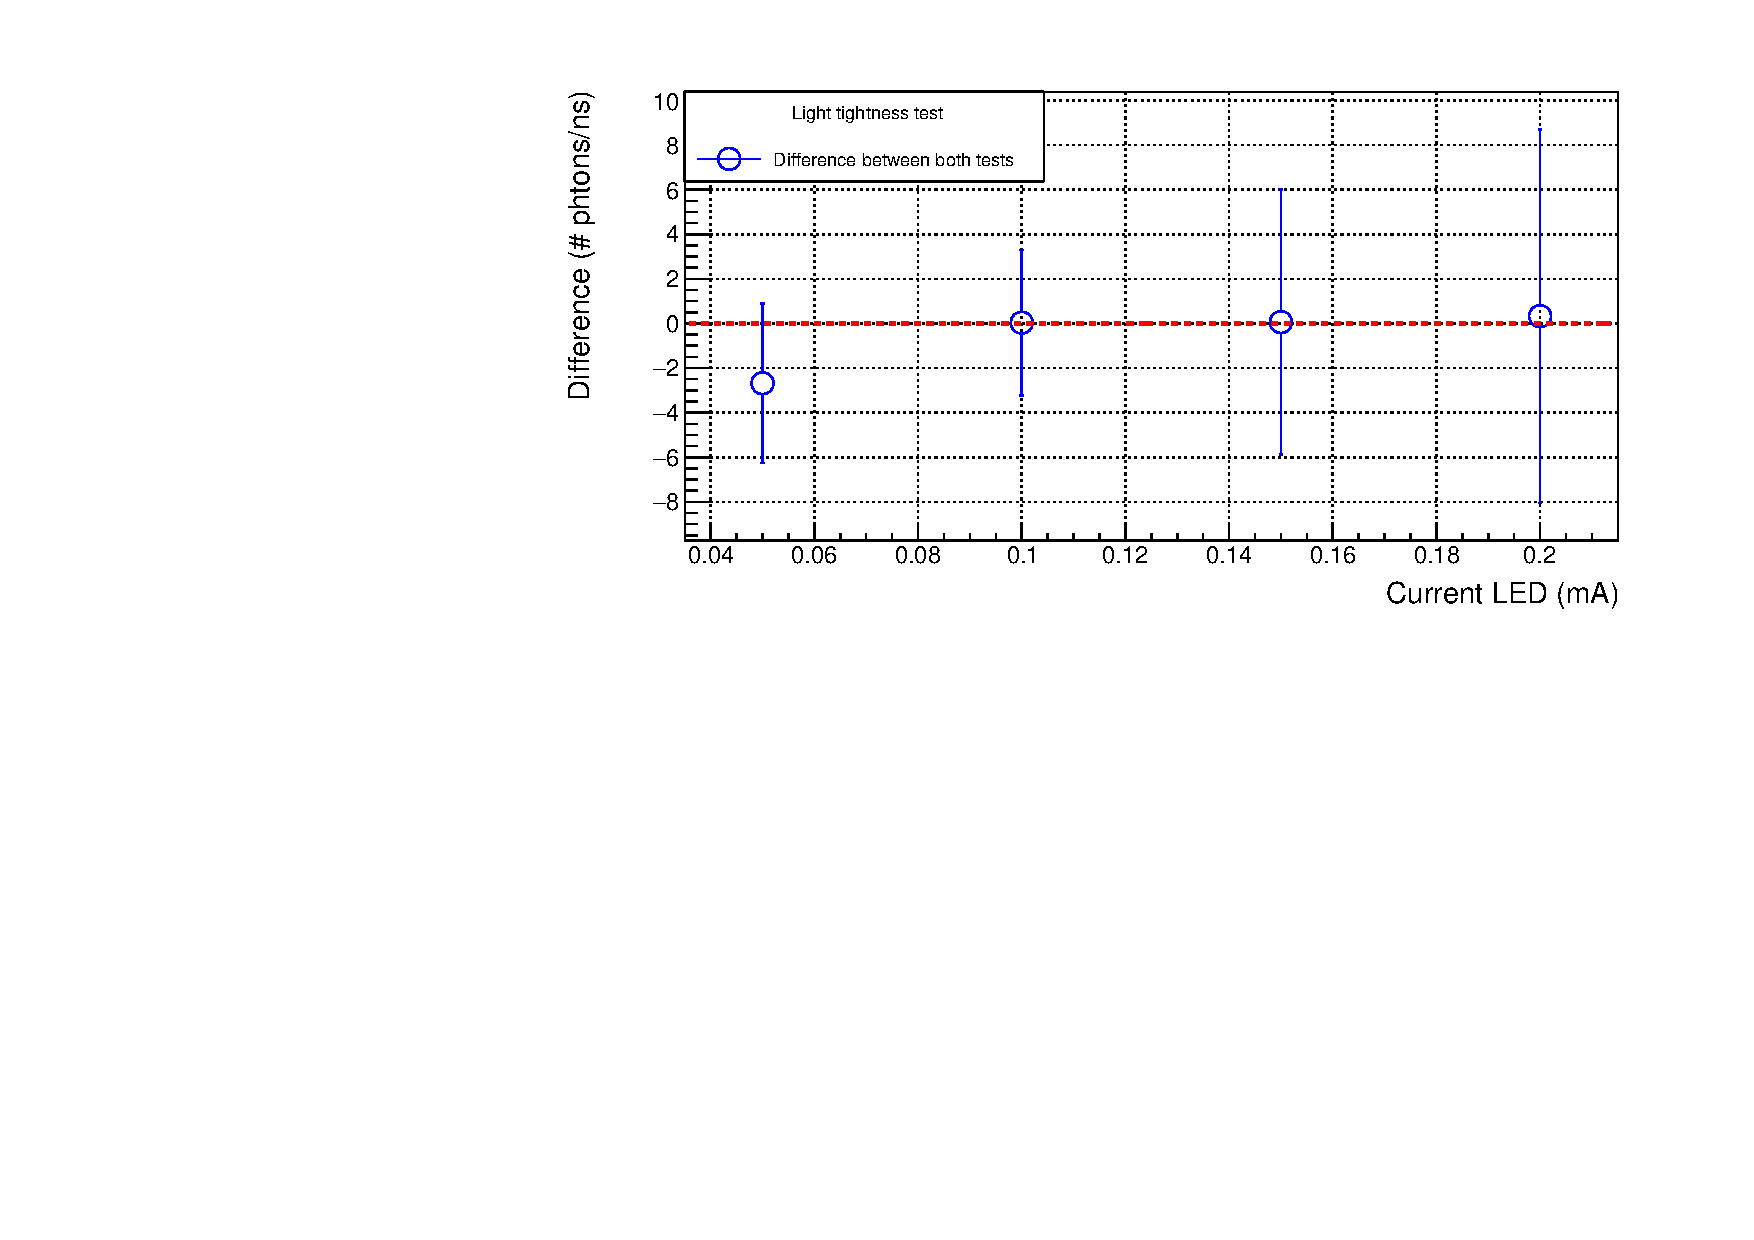
\includegraphics[width=0.9\textwidth]{4ResearchAndDevelopments/41Fibers/Light_tightness_difference.pdf}}
 %\caption{Energy spectrums used to test the effect of the Polishing machine}
 %\label{fig:LightTightnessTest}
%\end{figure}

\begin{figure}[h]
\centering
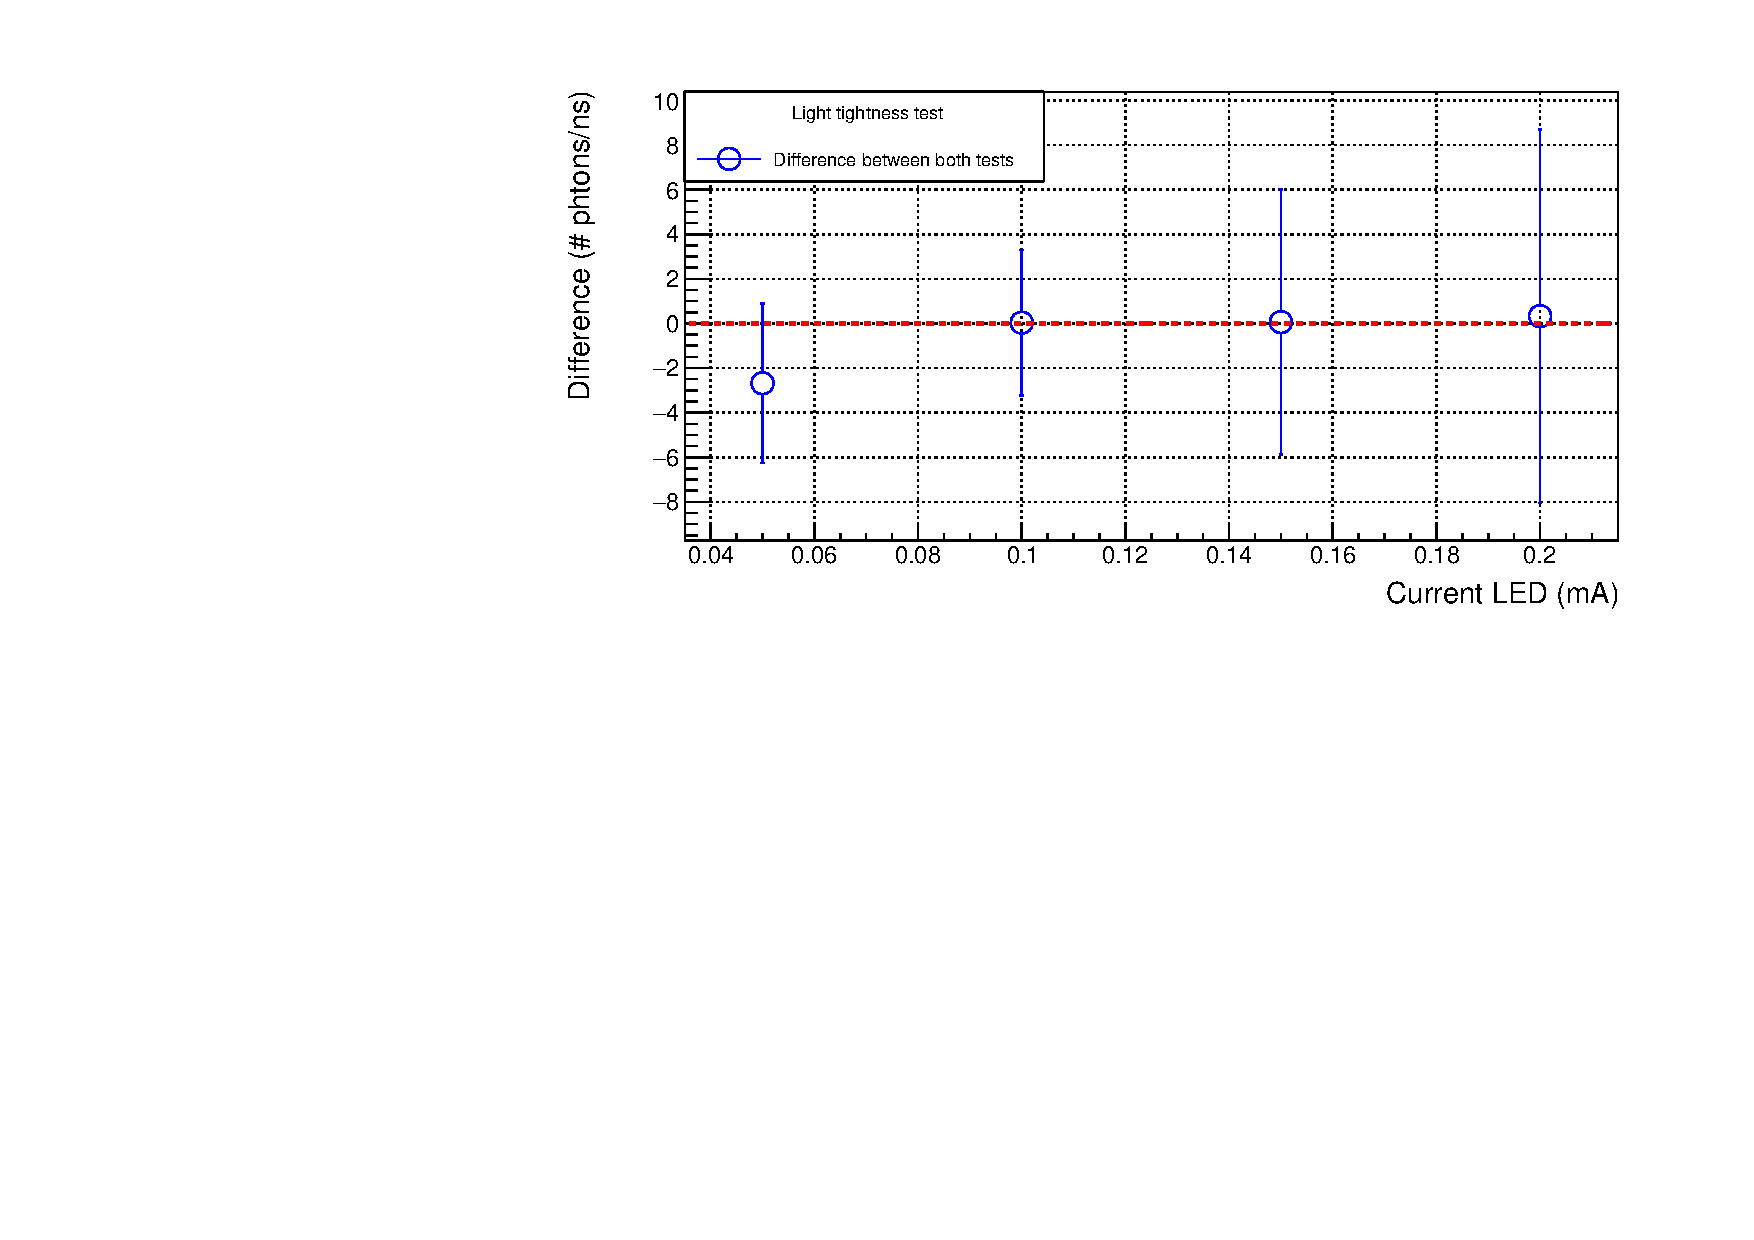
\includegraphics[scale=0.6]{4ResearchAndDevelopments/41Fibers/Light_tightness_difference.pdf}
\caption{Difference between the results obtained in both tests carried out to check the light-tight quality of the system.\label{fig:LightTightnessTest}}
\end{figure}

As can be seen in this figure, there are no statistically relevant differences between both situations, which can be verified with the help of the red auxiliary line that marks 0 (no difference). Therefore, it can be ensured that the quality of the light tightness of the black box used is high enough for this study.

Then the operation of the PCB without the internal gain will be verified. It consists of finding the plateau in which the electron collection efficiency in the first dynode is practically $100\%$. 

This test consists of, using the setup previously explained without any fiber, feeding the LED at $1~\milli\ampere$ intensity. There, the PMT output current was measured for different supply voltages of the PMT, between $0$ and $500~\volt$. The Figure \ref{fig:PlateauNoGainPMT} show the number of photons detected by the PMT (using a semi logarithmic scale).

\begin{figure}[h]
\centering
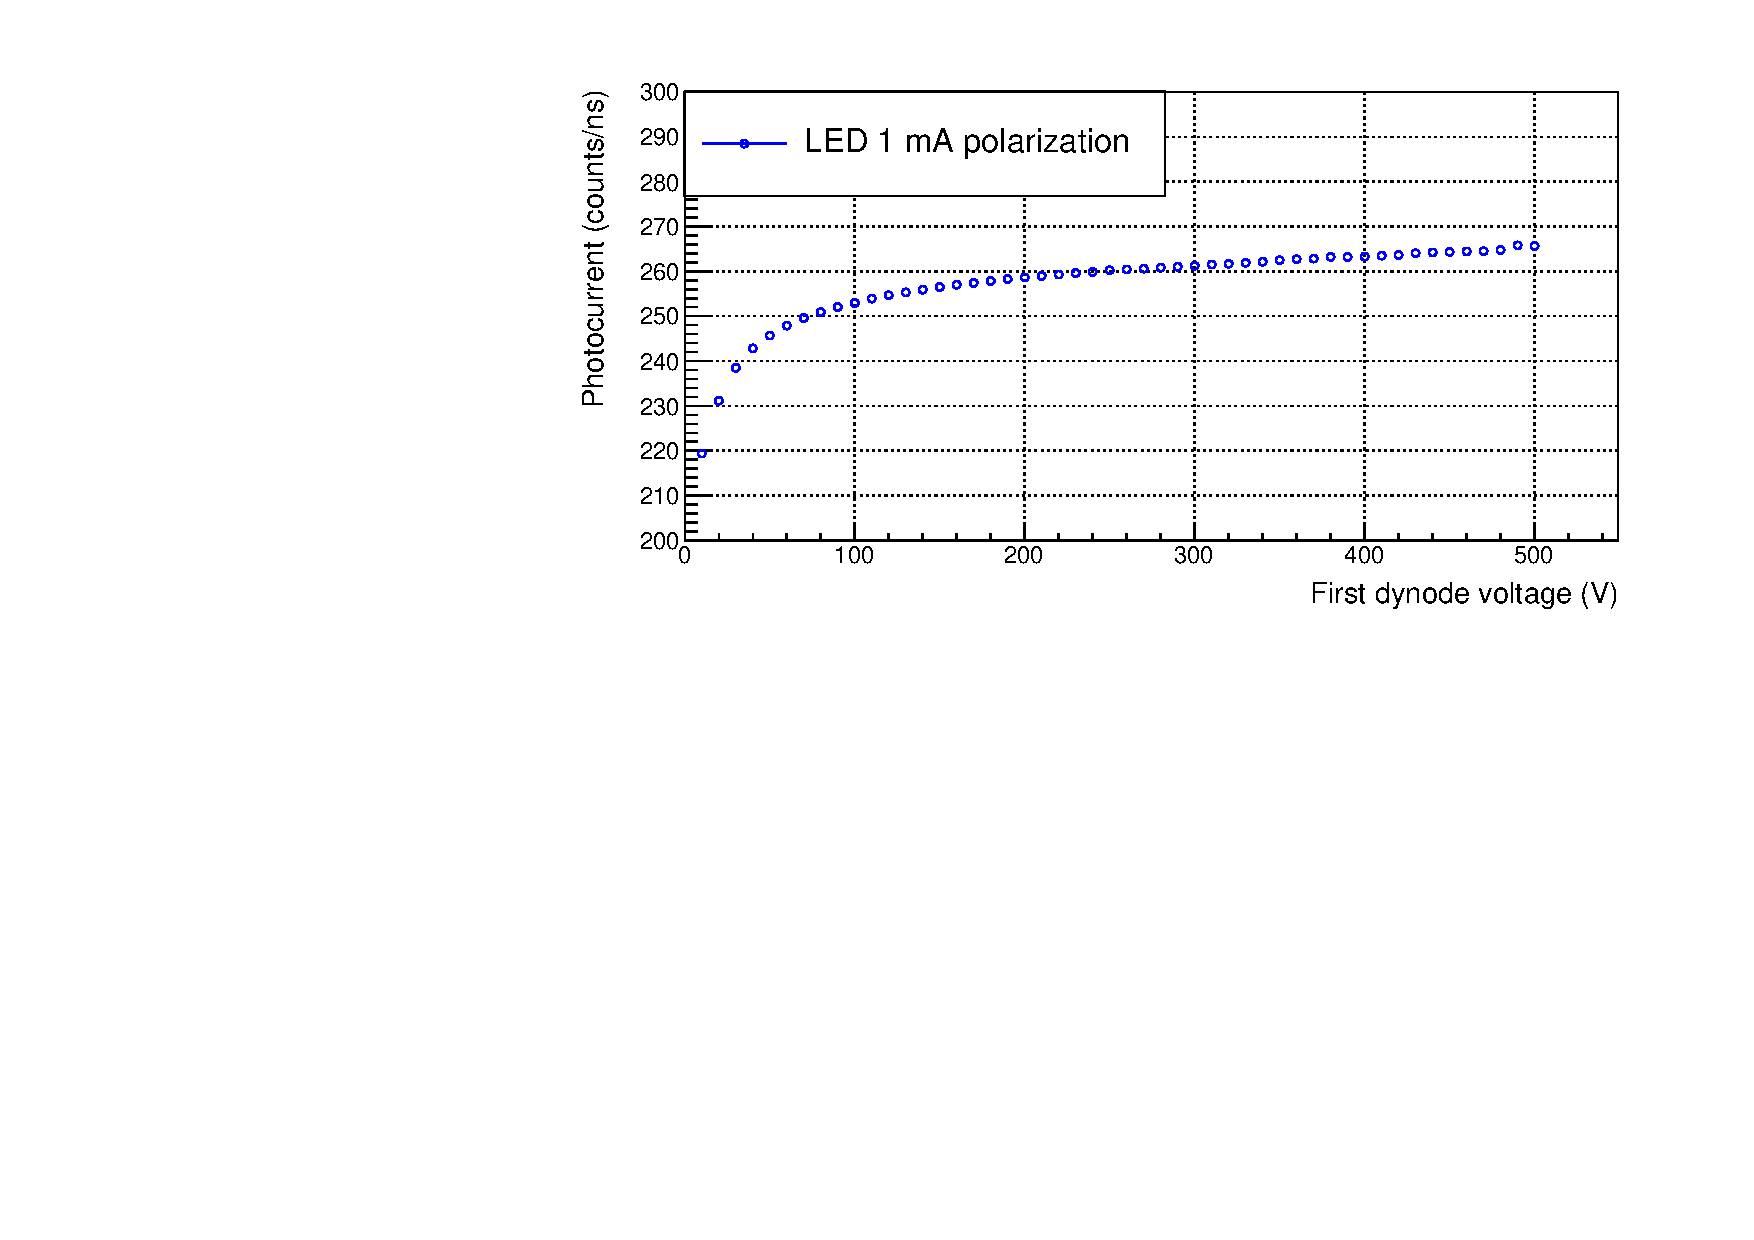
\includegraphics[scale=0.6]{4ResearchAndDevelopments/41Fibers/PCBNoGainPlateau_Calibrated.pdf}
\caption{Response of the PMT based on its high voltage using the PCB with which we get no internal gain from the PMT.\label{fig:PlateauNoGainPMT}}
\end{figure}

As can be seen, this plateau is found at voltages higher than $150~\volt$, where the PMT output response are stable. This is the interesting range for this study so, the chosen voltage at which this study was developed is $250~\volt$.

Finally, the linearity of the PMT is verified. In this study the LED will be powered with several intensities of up to $10~\milli\ampere$ (LED linearity range) to ensure that its emission is not saturated.

This linearity is tested in two different ranges, one in the range of the number of photons expected in a tritium event that is only a few tens of photons per tritium event (tens of photons per nanosecond), and second, in the range of this study, whose events will have up to two thousand five hundred photons per nanosecond.

To test the linearity of the PMT at the level of tritium events, the set up explained above is used without any fibers and without the connector that there is in the part of the PMT but keeping the collimators to ensure that the active area of the PMT is the same as the one we use in the study. 

To test the linearity of the PMT at the level of more than a thousand photons per nanosecond, we remove the other connector (the one in the LED part) in order to increase the photons emitted by the LED that reach the photosensor and also keeping the collimators.

Both results is shown in Figures \ref{fig:LinearityRangesOfPMT}, where the uncertainties are included but they are too small to be visible.

\begin{figure}[h]
 \centering
  \subfloat[Verification of linearity in the response of the PMT in the range of tritium events.]{
   \label{subfig:LinearityTritiumRange}
    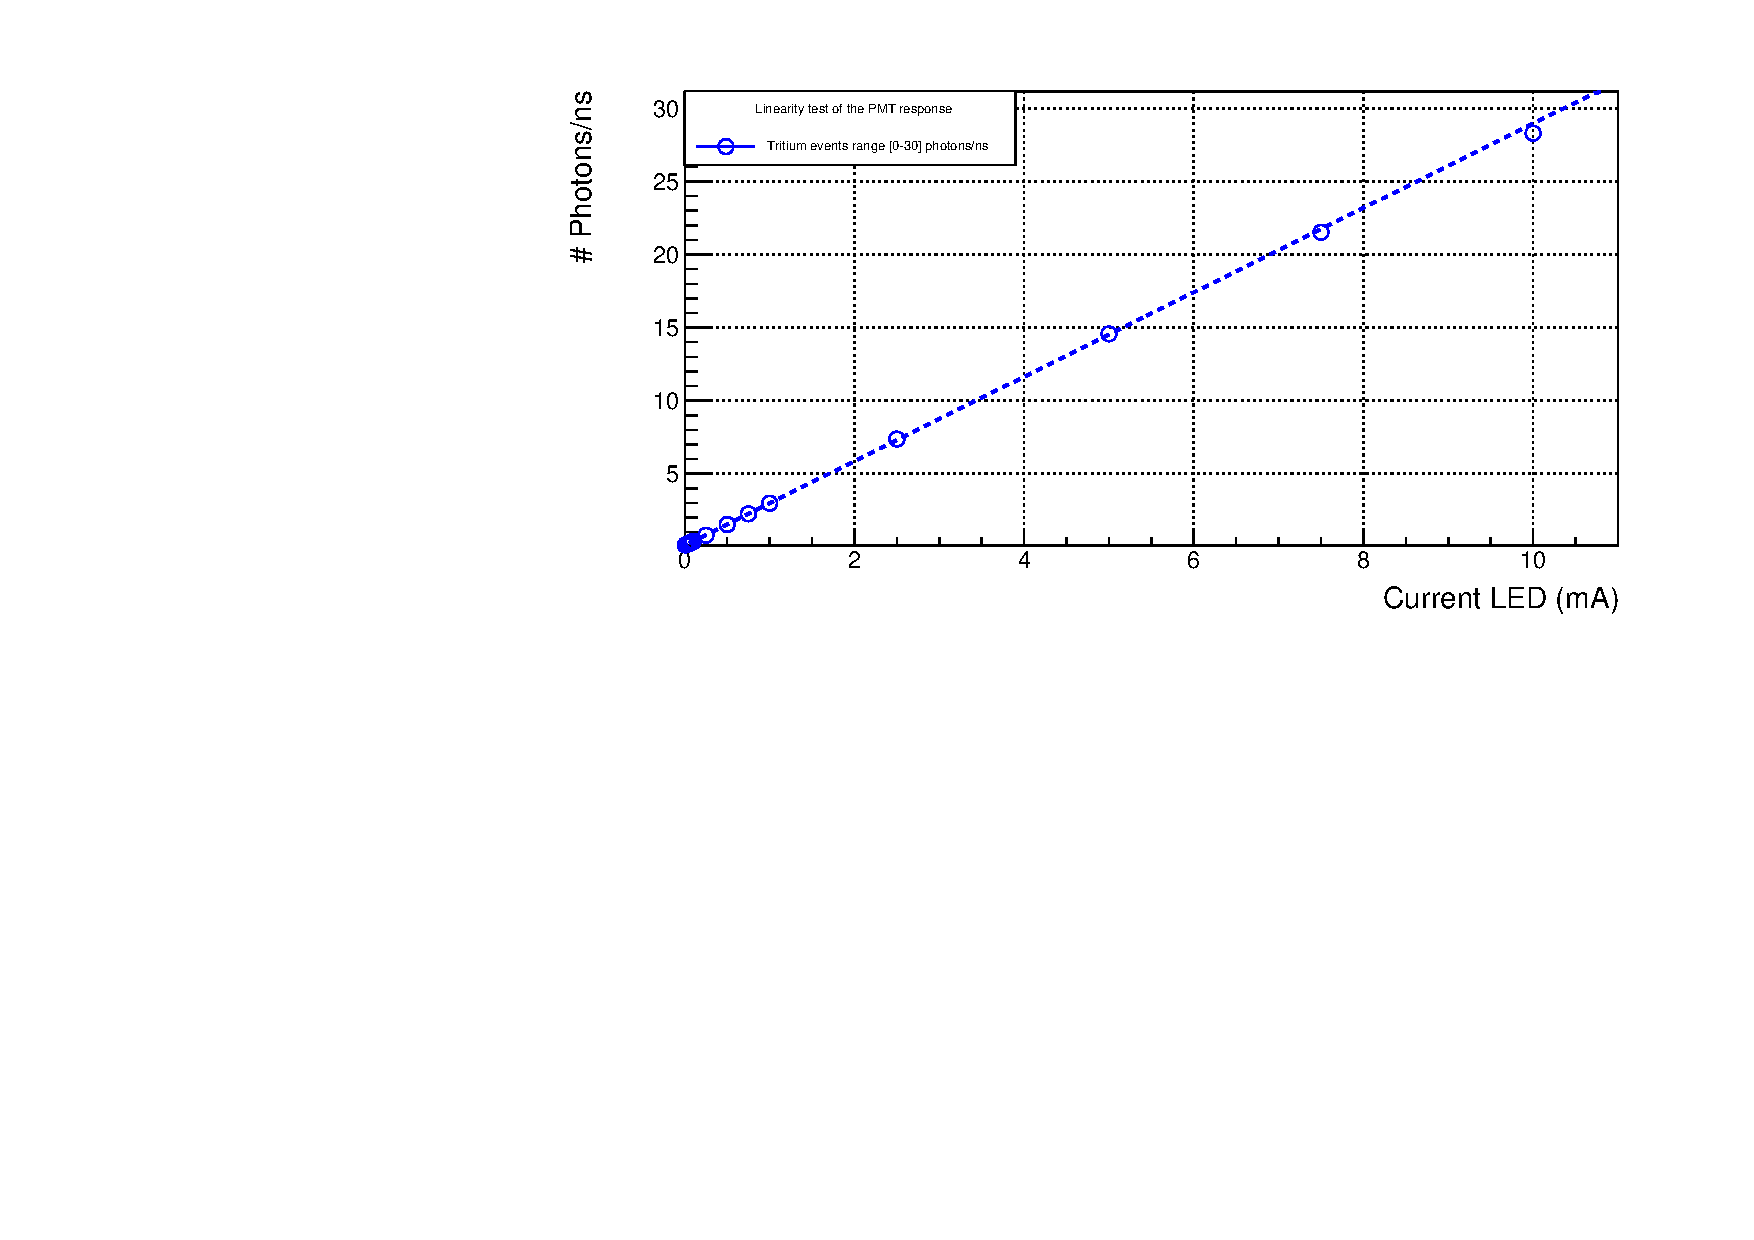
\includegraphics[width=0.7\textwidth]{4ResearchAndDevelopments/41Fibers/Linearity_test_0_30_range.pdf}}
    \newline
  \subfloat[Verification of linearity in the response of the PMT in the range of this study  $(0-2500)~\gamma/\nano\second$.]{
   \label{subfig:LinearityStudyRange}
    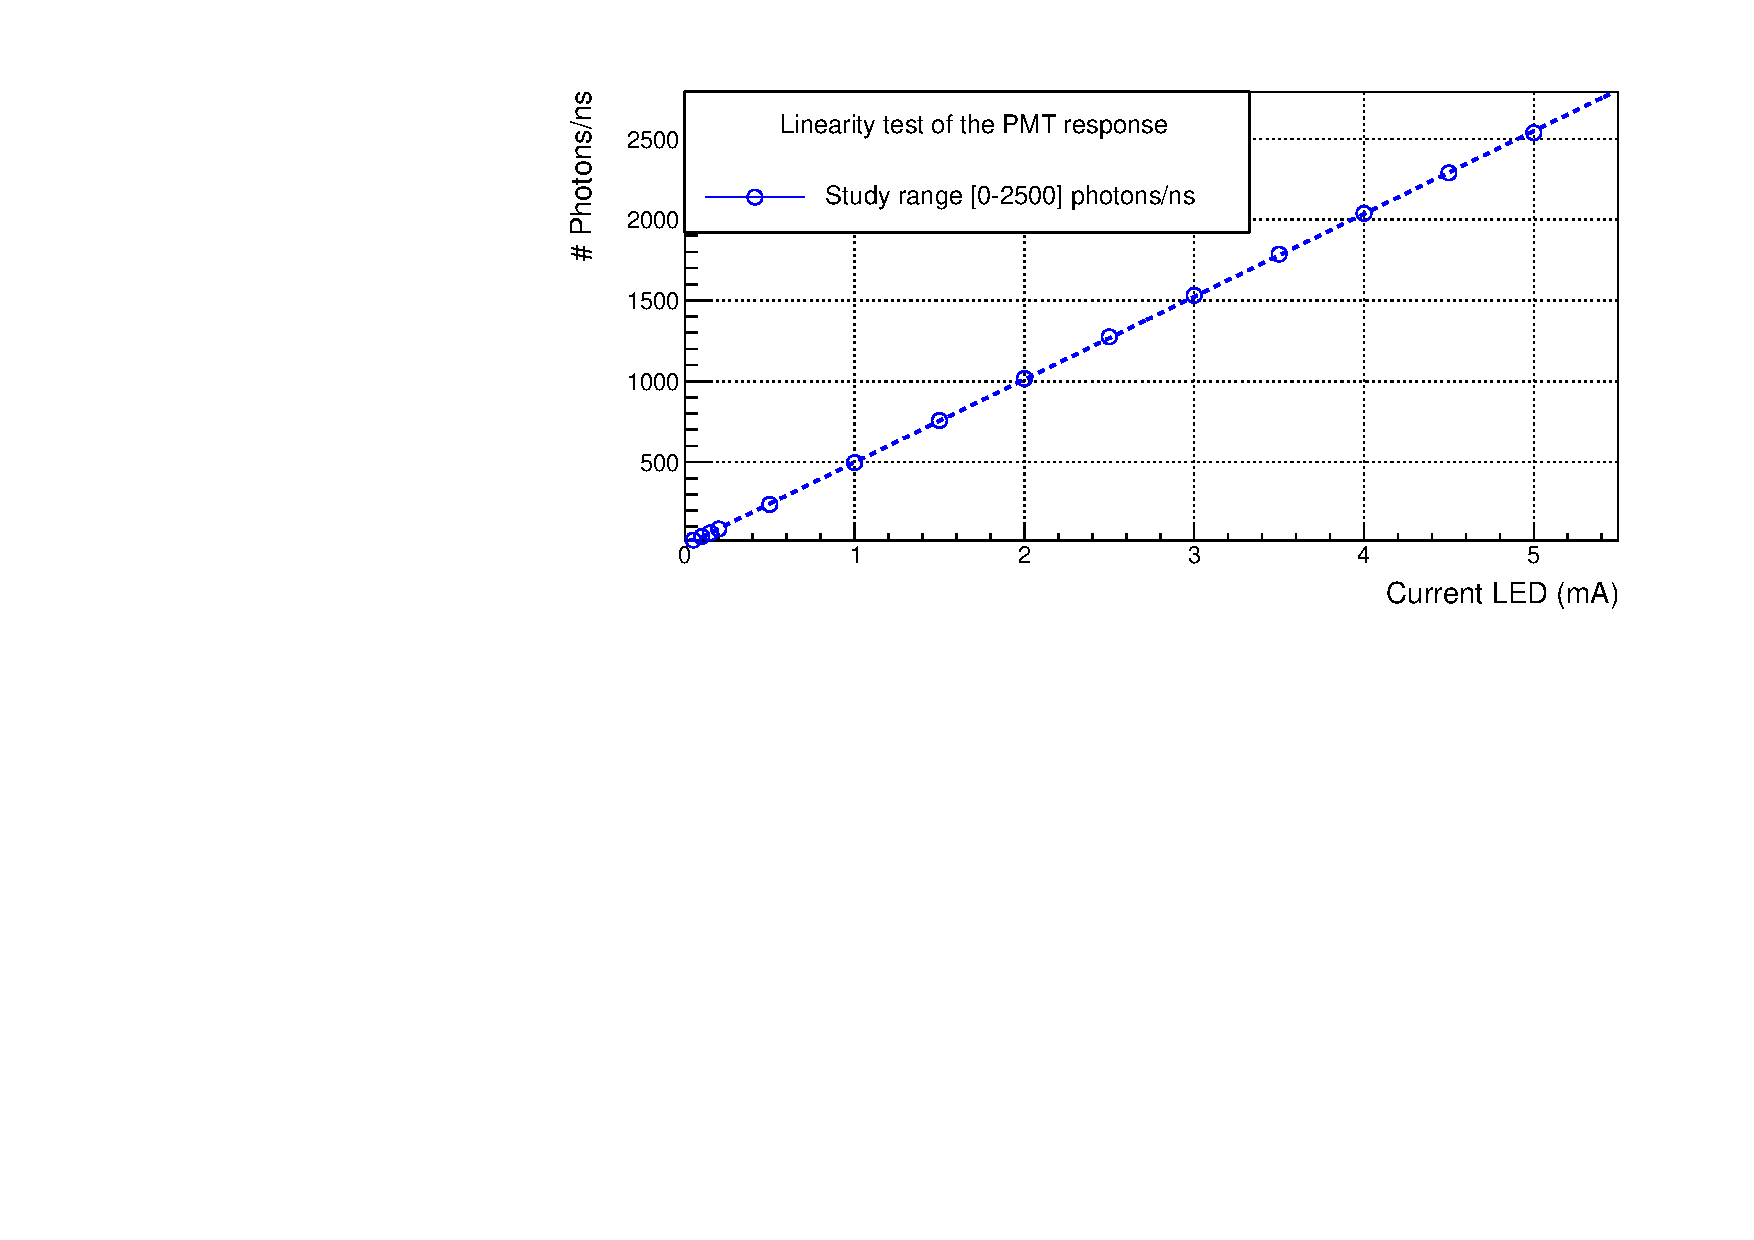
\includegraphics[width=0.7\textwidth]{4ResearchAndDevelopments/41Fibers/Linearity_test_0_2500_range.pdf}}
 \caption{Linearity tests of the PMT response}
 \label{fig:LinearityRangesOfPMT}
\end{figure}

As can be seen, the PMT output current is linear in both cases, so the system is ready to start with the characterization of the fibers.